%% ============================================================
%%  Rapport final — Contrôle d'un jeu par gestes de la main
%%  Vision par Ordinateur — Master 2 Mathématiques
%%  Auteurs : Christ Bohou  &  Djafarou Oulare
%%  Date   : Mars 2026
%% ============================================================
\documentclass[12pt,a4paper]{article}

% --- Encodage & langue ---
\usepackage[utf8]{inputenc}
\usepackage[T1]{fontenc}
\usepackage[french]{babel}
\usepackage{lmodern}

% --- Mise en page ---
\usepackage[top=2.5cm,bottom=2.5cm,left=2.8cm,right=2.8cm]{geometry}
\usepackage{setspace}
\onehalfspacing
\usepackage{parskip}

% --- Graphiques & couleurs ---
\usepackage{graphicx}
\usepackage[dvipsnames,table]{xcolor}
\usepackage{tikz}
\usetikzlibrary{shapes.geometric,arrows.meta,positioning,fit,backgrounds}
\usepackage{pgfplots}
\pgfplotsset{compat=1.18}

% --- Tableaux ---
\usepackage{booktabs}
\usepackage{multirow}
\usepackage{array}
\usepackage{tabularx}
\usepackage{diagbox}
\setlength{\headheight}{15pt}

% --- Maths ---
\usepackage{amsmath,amssymb}

% --- Code ---
\usepackage{listings}
\lstset{
  basicstyle=\ttfamily\small,
  backgroundcolor=\color{gray!8},
  frame=single,
  rulecolor=\color{gray!40},
  breaklines=true,
  showstringspaces=false,
  commentstyle=\color{gray},
  keywordstyle=\color{blue!70}\bfseries,
  stringstyle=\color{orange!80!black},
  numbers=left,
  numberstyle=\tiny\color{gray},
  xleftmargin=1.5em,
  language=Python
}

% --- Liens ---
\usepackage[hidelinks]{hyperref}

% --- En-têtes ---
\usepackage{fancyhdr}
\pagestyle{fancy}
\fancyhf{}
\rhead{\small Vision par Ordinateur — M2 Mathématiques}
\lhead{\small Contrôle d'un jeu par gestes de la main}
\cfoot{\thepage}

% --- Titres colorés ---
\usepackage{titlesec}
\titleformat{\section}{\large\bfseries\color{NavyBlue}}{\thesection}{1em}{}
\titleformat{\subsection}{\normalsize\bfseries\color{MidnightBlue}}{\thesubsection}{1em}{}

% --- Boîtes ---
\usepackage{tcolorbox}
\tcbuselibrary{skins,breakable}
\newtcolorbox{keybox}[1][]{colback=NavyBlue!5,colframe=NavyBlue!60,title=#1,fonttitle=\bfseries\small}
\newtcolorbox{resultbox}[1][]{colback=ForestGreen!5,colframe=ForestGreen!50,title=#1,fonttitle=\bfseries\small}
\newtcolorbox{failbox}[1][]{colback=BrickRed!5,colframe=BrickRed!50,title=#1,fonttitle=\bfseries\small}

%% ============================================================
\begin{document}
%% ============================================================

% ---- PAGE DE TITRE ----
\begin{titlepage}
\centering
\vspace*{1cm}

{\Huge\bfseries\color{NavyBlue}
Contrôle d'un Jeu Vidéo\\[0.3em]
par Gestes de la Main\par}

\vspace{0.8cm}
\rule{0.6\linewidth}{1.5pt}
\vspace{0.4cm}

{\large\itshape
Vision par Ordinateur — Cours d'Initiation\\
Master 2 Mathématiques\par}

\vspace{1.5cm}

\begin{tikzpicture}
\node[draw=NavyBlue,rounded corners=8pt,fill=NavyBlue!5,
      minimum width=10cm,minimum height=2.2cm,align=center,
      font=\large] at (0,0)
  {Webcam $\longrightarrow$ MediaPipe $\longrightarrow$ CNN $\longrightarrow$ WebSocket $\longrightarrow$ Jeu};
\end{tikzpicture}

\vspace{1.5cm}

{\large
\begin{tabular}{ll}
\textbf{Auteurs} & Christ Bohou \\
                 & Djafarou Oulare \\[0.5em]
\textbf{Date}   & Mars 2026
\end{tabular}\par}

\vfill
{\small Ce rapport décrit le pipeline complet de reconnaissance de gestes
en temps réel appliqué au jeu Space Invaders, depuis la collecte des données
jusqu'à l'intégration dans le navigateur.}
\end{titlepage}

% ---- TABLE DES MATIÈRES ----
\tableofcontents
\newpage

%% ============================================================
\section{Introduction et Objectif}
%% ============================================================

Ce projet s'inscrit dans le cadre du cours d'initiation à la Vision par Ordinateur
du Master 2 Mathématiques. L'objectif est de concevoir un système complet de
\textbf{reconnaissance de gestes de la main en temps réel} et de l'utiliser pour
contrôler le jeu classique \textit{Space Invaders} dans un navigateur web.

Le système repose sur une chaîne de traitement composée de quatre maillons :

\begin{enumerate}
  \item \textbf{Capture vidéo} : webcam standard à 30 images/seconde.
  \item \textbf{Détection de la main} : le modèle MediaPipe HandLandmarker
        extrait 21 points anatomiques en temps réel.
  \item \textbf{Classification} : un réseau de neurones dense classifie
        le vecteur de 63 coordonnées normalisées en l'un des 5 gestes du jeu.
  \item \textbf{Transmission} : les commandes sont envoyées via WebSocket
        (Node.js) au jeu JavaScript s'exécutant dans le navigateur.
\end{enumerate}

\begin{keybox}[Gestes reconnus — version finale]
\begin{center}
\begin{tabular}{clc}
\toprule
\textbf{Geste} & \textbf{Description} & \textbf{Commande} \\
\midrule
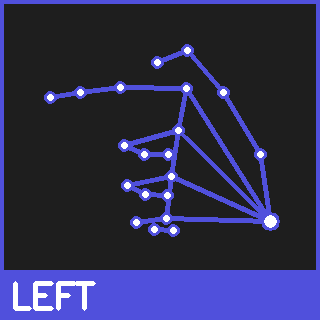
\includegraphics[height=1.2cm]{cnn_training/modeles/images_rapport/LEFT.png}
  & Main droite, index pointé vers la gauche & \texttt{LEFT} \\
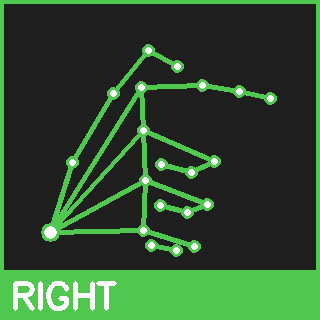
\includegraphics[height=1.2cm]{cnn_training/modeles/images_rapport/RIGHT.png}
  & Main gauche, index pointé vers la droite & \texttt{RIGHT} \\
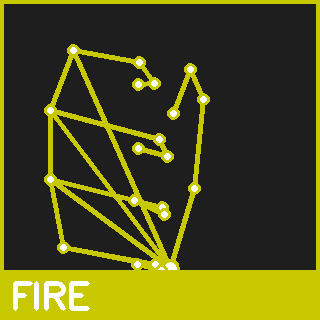
\includegraphics[height=1.2cm]{cnn_training/modeles/images_rapport/FIRE.png}
  & Poing fermé (knuckles face caméra) & \texttt{FIRE} \\

\includegraphics[height=1.2cm]{cnn_training/modeles/images_rapport/ENTER.png}
  & Main gauche, paume ouverte face caméra & \texttt{ENTER} \\
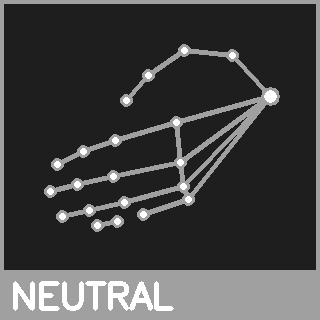
\includegraphics[height=1.2cm]{cnn_training/modeles/images_rapport/NEUTRAL.png}
  & Main au repos & \texttt{NEUTRAL} \\
\bottomrule
\end{tabular}
\end{center}
\end{keybox}

%% ============================================================
\section{Architecture Globale du Système}
%% ============================================================

\subsection{Vue d'ensemble}

\begin{figure}[h]
\centering
\begin{tikzpicture}[
  node distance=0.6cm and 0.5cm,
  box/.style={draw=NavyBlue,fill=NavyBlue!8,rounded corners=5pt,
              minimum width=2.8cm,minimum height=1cm,align=center,font=\small},
  arr/.style={-{Latex},thick,color=NavyBlue!70},
  label/.style={font=\tiny\itshape,color=gray}
]
\node[box] (cam)    {Webcam\\30 fps};
\node[box,right=of cam] (mp)  {MediaPipe\\HandLandmarker};
\node[box,right=of mp]  (cnn) {Réseau dense\\(TensorFlow)};
\node[box,right=of cnn] (ws)  {WebSocket\\Node.js};
\node[box,right=of ws]  (jeu) {Jeu\\(JavaScript)};

\draw[arr] (cam) -- node[above,label]{BGR→RGB} (mp);
\draw[arr] (mp)  -- node[above,label]{63 coords} (cnn);
\draw[arr] (cnn) -- node[above,label]{classe} (ws);
\draw[arr] (ws)  -- node[above,label]{keydown} (jeu);
\end{tikzpicture}
\caption{Pipeline de contrôle gestuel temps réel.}
\end{figure}

\subsection{Rôle de chaque composant}

\paragraph{MediaPipe HandLandmarker.}
Modèle pré-entraîné de Google basé sur une architecture MobileNet légère.
Il détecte la main avec BlazePalm puis prédit les coordonnées $(x, y, z)$
de 21 points anatomiques (poignet, phalanges) en mode \texttt{VIDEO},
ce qui permet un suivi temporel efficace entre les images.

\paragraph{Réseau de neurones dense.}
Le vecteur de 63 coordonnées normalisées est classifié par un réseau entraîné
sur nos propres données. Ce choix — travailler sur les \emph{landmarks} plutôt
que sur les pixels bruts — est la décision architecturale centrale du projet.

\paragraph{Serveur WebSocket Node.js.}
Un serveur \texttt{ws://localhost:8765} reçoit les commandes Python et les
traduit en événements clavier pour le navigateur via un mécanisme de
\emph{hold timer} (180\,ms) : la touche reste enfoncée tant que la commande
arrive, puis se lève automatiquement.

%% ============================================================
\section{Collecte et Préparation des Données}
%% ============================================================

\subsection{Approche 1 : images brutes (64×64 pixels)}

La première tentative a consisté à collecter directement des \textbf{images RGB}
de 64×64 pixels pour chaque geste. Le script \texttt{1\_collecter\_images.py}
capture automatiquement une image toutes les 300\,ms pendant 3 à 4 minutes par
classe.

\begin{center}
\begin{tabular}{lc}
\toprule
\textbf{Classe} & \textbf{Nombre d'images} \\
\midrule
LEFT    & 502 \\
RIGHT   & 516 \\
FIRE    & 520 \\
ENTER   & 520 \\
NEUTRAL & 463 \\
\midrule
\textbf{Total} & \textbf{2\,521} \\
\bottomrule
\end{tabular}
\end{center}

\subsection{Approche 2 : landmarks normalisés (vecteur 63D)}

La seconde approche — retenue — extrait les 21 landmarks MediaPipe
et les normalise en un vecteur de 63 valeurs réelles.

\paragraph{Normalisation.} Pour chaque frame, le vecteur brut $\mathbf{p} \in \mathbb{R}^{21 \times 3}$ est transformé :

\begin{equation}
  \tilde{\mathbf{p}} = \frac{\mathbf{p} - \mathbf{p}_0}{\max_i |\mathbf{p}_i - \mathbf{p}_0|}
\end{equation}

où $\mathbf{p}_0$ est la position du poignet (point 0). Cette normalisation rend la
représentation invariante à la \textbf{position} de la main dans le cadre,
à l'\textbf{échelle} (distance à la caméra), et à la \textbf{taille} de la main.

Le vecteur aplati $\tilde{\mathbf{p}} \in [-1, 1]^{63}$ est sauvegardé en CSV
avec sa classe. Environ 2\,100 échantillons ont été collectés à raison de
1 capture automatique toutes les 300\,ms.

\subsection{Approche de Djafarou : dataset Kaggle}

En parallèle, une seconde approche a été explorée sur un dataset externe Kaggle
(\emph{Hand Navigation Landmarks}, harisudhan411) contenant 8\,000 images
180×180 en 4 classes (left, right, up, down) sur fond contrôlé uniforme.

\begin{center}
\begin{tabular}{lccc}
\toprule
\textbf{Ensemble} & \textbf{Train} & \textbf{Validation} & \textbf{Test} \\
\midrule
Nombre d'images & 8\,000 & 400 & 1\,200 \\
\bottomrule
\end{tabular}
\end{center}

%% ============================================================
\section{Modèles de Classification}
%% ============================================================

\subsection{CNN sur images brutes — Approche 1 (Christ Bohou)}

\subsubsection{Architecture}

Un CNN à 3 blocs convolutifs a été construit avec augmentation de données
en ligne (\textit{data augmentation}) pour compenser la faible taille du dataset.

\begin{center}
\begin{tabular}{llcl}
\toprule
\textbf{Bloc} & \textbf{Couche} & \textbf{Filtres} & \textbf{Sortie} \\
\midrule
\multirow{4}{*}{Bloc 1}
  & Conv2D 3×3 ReLU (same) & 32  & 64×64×32 \\
  & BatchNormalization      & —   & 64×64×32 \\
  & Conv2D 3×3 ReLU (same) & 32  & 64×64×32 \\
  & MaxPooling2D 2×2        & —   & 32×32×32 \\
  & Dropout(0.25)           & —   & 32×32×32 \\
\midrule
\multirow{4}{*}{Bloc 2}
  & Conv2D 3×3 ReLU (same) & 64  & 32×32×64 \\
  & BatchNormalization      & —   & 32×32×64 \\
  & Conv2D 3×3 ReLU (same) & 64  & 32×32×64 \\
  & MaxPooling2D 2×2        & —   & 16×16×64 \\
  & Dropout(0.25)           & —   & 16×16×64 \\
\midrule
\multirow{3}{*}{Bloc 3}
  & Conv2D 3×3 ReLU (same) & 128 & 16×16×128 \\
  & BatchNormalization      & —   & 16×16×128 \\
  & MaxPooling2D 2×2        & —   & 8×8×128 \\
  & Dropout(0.25)           & —   & 8×8×128 \\
\midrule
\multirow{4}{*}{Tête dense}
  & Flatten                 & —   & 8\,192 \\
  & Dense(256) ReLU         & —   & 256 \\
  & BatchNormalization      & —   & 256 \\
  & Dropout(0.5)            & —   & 256 \\
  & Dense(5) Softmax        & —   & 5 \\
\bottomrule
\end{tabular}
\end{center}

\textbf{Paramètres entraînables : 2\,240\,037.}

\paragraph{Configuration d'entraînement.}
\begin{itemize}
  \item Optimiseur : Adam ($\eta = 10^{-3}$), perte : \textit{sparse\_categorical\_crossentropy}
  \item Batch : 32, max 30 epochs ; split 80/20
  \item Augmentation : flip horizontal, rotation ±15\%, zoom ±15\%,
        luminosité ±20\%, contraste ±20\%
  \item Callbacks : EarlyStopping (patience=8), ReduceLROnPlateau (factor=0.5, patience=4)
\end{itemize}

\subsubsection{Résultats et analyse}

\begin{failbox}[Résultat — CNN images brutes]
\textbf{Meilleure val\_accuracy : 34.3\%} (époque 14 sur 22).
Précision chance aléatoire : 20\% (1 classe sur 5).
\end{failbox}

Le modèle n'apprend pas à généraliser. L'accuracy de validation stagne autour
de 20\% pendant la majeure partie de l'entraînement avec un pic isolé à 34\%.
\textbf{Cause principale} : le CNN apprend le fond de la pièce autant que la
main elle-même. Avec seulement 2\,521 images collectées dans un seul
environnement, le modèle sur-apprend les artefacts de fond. La moindre variation
d'éclairage ou de position dégrade les performances.

\subsection{Approche MLP et CNN sur images — Djafarou Oulare}

\subsubsection{MLP (Perceptron Multicouche)}

\begin{center}
\begin{tabular}{lc}
\toprule
\textbf{Couche} & \textbf{Unités} \\
\midrule
Flatten (180×180×3) & 97\,200 \\
Dense ReLU          & 128 \\
Dense Softmax       & 4 \\
\bottomrule
\end{tabular}
\end{center}

Entraîné sur 100 epochs avec Adam et \textit{categorical\_crossentropy}.
Les données sont normalisées pixel/255 et encodées en one-hot.

\subsubsection{CNN Kaggle}

\begin{center}
\begin{tabular}{lc}
\toprule
\textbf{Couche} & \textbf{Sortie} \\
\midrule
Rescaling(1/255)     & 180×180×3 \\
Conv2D(32, 3×3) ReLU & 178×178×32 \\
MaxPooling2D 2×2     & 89×89×32 \\
Conv2D(64, 3×3) ReLU & 87×87×64 \\
MaxPooling2D 2×2     & 43×43×64 \\
Flatten              & 118\,336 \\
Dense(128) ReLU      & 128 \\
Dropout(0.5)         & 128 \\
Dense(4) Softmax     & 4 \\
\bottomrule
\end{tabular}
\end{center}

\textbf{Paramètres : 15\,167\,044.} Ce modèle atteint 100\% de val\_accuracy
sur le dataset Kaggle (fond uniforme) mais \textbf{échoue en conditions réelles}
(webcam dans une pièce normale) en raison de son adaptation totale au fond
contrôlé du dataset.

\begin{failbox}[Limites des approches pixel]
Les deux approches image-based (CNN et MLP) souffrent du même problème :
elles apprennent le contexte visuel de fond autant que la forme de la main.
Un dataset entraîné dans un bureau ne fonctionne pas dans une autre pièce.
\end{failbox}

\subsection{Réseau Dense sur Landmarks — Solution Retenue (Christ Bohou)}

\subsubsection{Principe}

Plutôt que de traiter les pixels, on extrait d'abord les 21 landmarks
MediaPipe (représentation géométrique de la main), puis on entraîne un
réseau dense sur ces coordonnées normalisées. La représentation est
\textbf{invariante au fond, à la luminosité, à la couleur de peau et
à la taille de la main}.

\subsubsection{Architecture}

\begin{center}
\begin{tabular}{lcc}
\toprule
\textbf{Couche} & \textbf{Unités} & \textbf{Activation} \\
\midrule
Input       & 63  & — \\
Dense       & 128 & ReLU \\
BatchNorm   & 128 & — \\
Dropout     & 128 & — (taux : 0.3) \\
Dense       & 128 & ReLU \\
BatchNorm   & 128 & — \\
Dropout     & 128 & — (taux : 0.3) \\
Dense       & 64  & ReLU \\
BatchNorm   & 64  & — \\
Dropout     & 64  & — (taux : 0.2) \\
Dense       & 5   & Softmax \\
\bottomrule
\end{tabular}
\end{center}

\textbf{Paramètres entraînables : 33\,925} — soit \textbf{66 fois moins} que
le CNN images.

\paragraph{Configuration d'entraînement.}
Optimiseur Adam ($\eta = 10^{-3}$), perte sparse\_categorical\_crossentropy,
batch 32, max 50 epochs (EarlyStopping patience=15), ReduceLROnPlateau.

\subsubsection{Résultats}

\begin{resultbox}[Résultat — Réseau dense sur landmarks]
\textbf{Meilleure val\_accuracy : 99.6\%} (époque 13 sur 28).\\
2 erreurs sur 501 échantillons de validation.\\
Temps d'entraînement : < 30 secondes sur CPU.
\end{resultbox}

\begin{figure}[h]
\centering
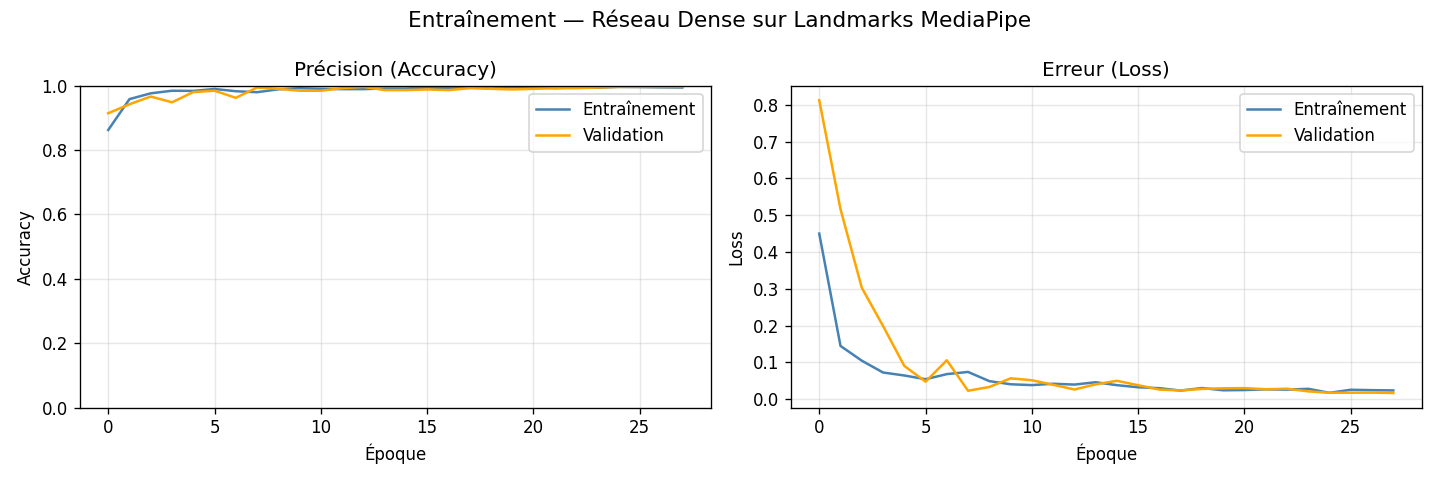
\includegraphics[width=0.85\textwidth]{cnn_training/modeles/courbes_landmarks.png}
\caption{Courbes d'entraînement du réseau dense sur landmarks.
La convergence est rapide et stable.}
\end{figure}

\paragraph{Matrice de confusion (501 échantillons de validation).}

\begin{center}
\begin{tabular}{l|ccccc}
\toprule
\diagbox{\textbf{Réel}}{\textbf{Prédit}} & ENTER & FIRE & LEFT & NEUTRAL & RIGHT \\
\midrule
ENTER   & \textbf{100} & 0 & 0 & 0 & 0 \\
FIRE    & 0 & \textbf{100} & 0 & 0 & 0 \\
LEFT    & 0 & 0 & \textbf{100} & 0 & 0 \\
NEUTRAL & 0 & 1 & 1 & \textbf{99} & 0 \\
RIGHT   & 0 & 0 & 0 & 0 & \textbf{100} \\
\bottomrule
\end{tabular}
\end{center}

Les 2 erreurs proviennent de la classe NEUTRAL, confondue une fois avec FIRE
et une fois avec LEFT. Ceci s'explique géométriquement : une main
en position de repos partielle ressemble à un poing ou à un index
semi-étendu.

%% ============================================================
\section{Comparaison des Approches}
%% ============================================================

\begin{table}[h]
\centering
\begin{tabularx}{\linewidth}{Xcccc}
\toprule
\textbf{Critère}
  & \textbf{CNN images}
  & \textbf{MLP Kaggle}
  & \textbf{CNN Kaggle}
  & \textbf{Dense landmarks} \\
\midrule
Val. accuracy        & 34.3\%      & N/A  & $\sim$100\%  & \textbf{99.6\%} \\
Perf. en conditions réelles & Mauvaise & Mauvaise & Mauvaise & \textbf{Bonne} \\
Paramètres           & 2.24M       & 12.5M & 15.2M & \textbf{33\,925} \\
Temps/epoch (CPU)    & $\sim$16\,s & $\sim$60\,s & $\sim$45\,s & \textbf{< 1\,s} \\
Données nécessaires  & 50\,000+    & 8\,000 (ext.) & 8\,000 (ext.) & \textbf{$\sim$2\,000} \\
Sensibilité au fond  & Critique   & Critique & Critique & \textbf{Nulle} \\
Invariant taille main & Non       & Non & Non & \textbf{Oui} \\
Dataset propre       & Oui        & Non (Kaggle) & Non (Kaggle) & \textbf{Oui} \\
\bottomrule
\end{tabularx}
\caption{Comparaison des quatre approches expérimentées.}
\end{table}

\subsection{Analyse de la représentation}

Le facteur déterminant de succès est le \textbf{choix de la représentation
de l'entrée}, pas la complexité du modèle.

En passant des pixels bruts (64×64×3 = 12\,288 dimensions, sensibles au fond)
aux landmarks normalisés (63 dimensions, invariants au fond), on :
\begin{itemize}
  \item réduit la dimensionnalité d'un facteur $\mathbf{195}$,
  \item élimine toute information de fond, de couleur et de taille,
  \item réduit les paramètres du modèle d'un facteur $\mathbf{66}$,
  \item améliore la val\_accuracy de $\mathbf{34.3\% \to 99.6\%}$.
\end{itemize}

Cette observation est un exemple concret du principe général en apprentissage
automatique : \textit{une bonne représentation vaut mieux qu'un grand modèle}.

%% ============================================================
\section{Intégration Temps Réel}
%% ============================================================

\subsection{Architecture logicielle}

\begin{figure}[h]
\centering
\begin{tikzpicture}[
  proc/.style={draw=NavyBlue,fill=NavyBlue!6,rounded corners,
               minimum width=3cm,minimum height=1.1cm,align=center,font=\small},
  srv/.style={draw=orange!70!black,fill=orange!8,rounded corners,
              minimum width=3cm,minimum height=1.1cm,align=center,font=\small},
  game/.style={draw=ForestGreen!70,fill=ForestGreen!6,rounded corners,
               minimum width=3cm,minimum height=1.1cm,align=center,font=\small},
  arr/.style={-{Latex},thick}
]
\node[proc] (py) {Python\\(OpenCV + MediaPipe\\+ TensorFlow)};
\node[srv,right=2cm of py] (node) {Node.js\\(serveur WebSocket\\port 8765)};
\node[game,right=2cm of node] (js) {JavaScript\\(Space Invaders\\port 8000)};

\draw[arr,color=NavyBlue] (py) -- node[above,font=\tiny]{\texttt{ws send(classe)}} (node);
\draw[arr,color=orange!70!black] (node) -- node[above,font=\tiny]{\texttt{keydown/keyup}} (js);
\end{tikzpicture}
\caption{Architecture trois processus du système de contrôle gestuel.}
\end{figure}

\subsection{Gestion du threading Python}

Le script \texttt{5\_jouer\_avec\_cnn.py} utilise une architecture bi-thread
pour éviter le blocage réseau :

\begin{itemize}
  \item \textbf{Thread principal} : capture OpenCV + inférence MediaPipe + CNN
        (traitement synchrone, ~ 30 fps)
  \item \textbf{Thread WebSocket} : lecture de la file \texttt{Queue} et envoi
        des commandes (non-bloquant grâce à \texttt{put\_nowait})
\end{itemize}

\begin{lstlisting}[caption={Communication inter-threads par file de messages.}]
commande_queue = queue.Queue(maxsize=20)

# Thread principal : rempli la file
commande_queue.put_nowait({'type': geste})

# Thread WS : vide la file
msg = commande_queue.get(timeout=0.1)
ws.send(json.dumps(msg))
\end{lstlisting}

\subsection{Hold Timer dans le serveur Node.js}

Le jeu JavaScript génère des événements clavier (\texttt{keydown}/\texttt{keyup}).
Or Python envoie des commandes discrètes (à intervalle irrégulier), pas des
états continus. Le serveur Node.js résout ce découplage avec un \textbf{hold
timer} de 180\,ms :

\begin{itemize}
  \item À la réception de \texttt{LEFT}, le serveur envoie \texttt{keydown(37)}.
  \item Si aucune nouvelle commande \texttt{LEFT} n'arrive dans les 180\,ms,
        il envoie \texttt{keyup(37)}.
  \item Chaque nouvelle commande réinitialise le timer, maintenant la touche
        enfoncée tant que le geste est détecté.
\end{itemize}

Ce mécanisme permet un mouvement fluide continu même avec une reconnaissance
à 30 fps.

\subsection{Cooldowns et seuil de confiance}

Pour éviter les faux positifs et les commandes parasites :

\begin{center}
\begin{tabular}{lcc}
\toprule
\textbf{Commande} & \textbf{Cooldown} & \textbf{Seuil confiance} \\
\midrule
LEFT  & 80\,ms   & 70\% \\
RIGHT & 80\,ms   & 70\% \\
FIRE  & 80\,ms   & 70\% \\
ENTER & 800\,ms  & 70\% \\
NEUTRAL & — (jamais envoyé) & — \\
\bottomrule
\end{tabular}
\end{center}

%% ============================================================
\section{Résultats et Analyse Critique}
%% ============================================================

\subsection{Performance en conditions réelles}

Le réseau dense sur landmarks atteint \textbf{99.6\% en validation}
et \textbf{fonctionne de manière fiable en temps réel} sur webcam dans
des conditions d'éclairage variées. Les gestes LEFT, RIGHT, ENTER et NEUTRAL
sont reconnus sans erreur notable. Le geste FIRE (poing fermé) présente
une légère ambiguïté quand la main est semi-fermée (transition vers NEUTRAL).

\subsection{Limites identifiées}

\begin{enumerate}
  \item \textbf{FIRE entraîné sur une seule main.} Les données de collecte
        ont été capturées principalement avec la main gauche. Le modèle
        reconnaît moins bien le même geste effectué avec la main droite,
        car les landmarks sont symétriques (coordonnées $x$ inversées)
        et constituent une forme différente pour le réseau.

  \item \textbf{Impossibilité de tirer en se déplaçant.} La classification
        étant unimodale (une classe par frame), le système ne peut envoyer
        qu'une commande à la fois. Il est impossible de prédire simultanément
        LEFT et FIRE.

  \item \textbf{Latence} : la chaîne complète (capture → MediaPipe → CNN →
        WebSocket → jeu) introduit environ 40 à 80\,ms de latence,
        imperceptible en gameplay normal.

  \item \textbf{Dépendance à MediaPipe.} Si la main sort du cadre ou est
        partiellement occultée, MediaPipe ne détecte rien et aucune commande
        n'est envoyée (comportement sûr mais parfois gênant).
\end{enumerate}

%% ============================================================
\section{Perspectives d'Amélioration}
%% ============================================================

\subsection{Court terme : commandes simultanées}

La limitation la plus impactante sur la jouabilité est l'impossibilité de
tirer en se déplaçant. Une solution est d'ajouter 2 classes composites :

\begin{center}
\begin{tabular}{lll}
\toprule
\textbf{Classe} & \textbf{Geste} & \textbf{Commandes envoyées} \\
\midrule
\texttt{LEFT\_FIRE}  & Poing incliné à gauche & LEFT + FIRE \\
\texttt{RIGHT\_FIRE} & Poing incliné à droite & RIGHT + FIRE \\
\bottomrule
\end{tabular}
\end{center}

La transition \texttt{LEFT} $\to$ \texttt{LEFT\_FIRE} consiste à fermer
le poing sans bouger le bras — geste naturel et peu fatigant.

\subsection{Moyen terme : robustesse du geste FIRE}

Collecter le geste FIRE avec \textbf{les deux mains} à parts égales.
Les landmarks de la main droite étant le miroir de la gauche
(coordonnée $x \to -x$), on peut aussi faire de l'augmentation de données
par réflexion sans recollecte.

\subsection{Long terme : architecture plus expressive}

\begin{itemize}
  \item \textbf{LSTM ou Transformer temporel} : encoder non plus une frame
        mais une séquence de 5 à 10 frames de landmarks. Cela permettrait
        de reconnaître des \emph{gestes dynamiques} (main qui se déplace
        vers la droite, pas juste pointée à droite) et d'éliminer les
        faux positifs de transition.

  \item \textbf{Deux mains simultanées} : MediaPipe supporte jusqu'à 2 mains.
        En traitant les deux, on pourrait par exemple : main gauche = direction,
        main droite = tir, ce qui résout le problème de simultanéité
        de manière naturelle.
\end{itemize}

%% ============================================================
\section{Conclusion}
%% ============================================================

Ce projet a permis de concevoir et déployer un pipeline complet de
reconnaissance de gestes en temps réel, depuis la capture webcam jusqu'au
contrôle d'un jeu dans le navigateur. Il illustre plusieurs concepts
fondamentaux de la vision par ordinateur et de l'apprentissage automatique :

\begin{itemize}
  \item \textbf{L'importance de la représentation} : le choix des landmarks
        normalisés plutôt que des pixels bruts a été le facteur décisif,
        faisant passer la précision de 34.3\% à 99.6\% avec un modèle
        66 fois plus petit.

  \item \textbf{La généralisation} : un modèle entraîné sur un dataset
        externe (Kaggle, fond contrôlé) ne transfère pas en conditions
        réelles. Nos propres données, bien que moins nombreuses, donnent
        un modèle qui fonctionne dans notre environnement.

  \item \textbf{L'ingénierie système} : la performance perçue dépend autant
        du modèle que de l'architecture (threading, WebSocket, hold timer).
        Un bon modèle mal intégré donne une mauvaise expérience utilisateur.

  \item \textbf{Les limites honnêtes} : le système ne permet pas encore de
        tirer en se déplaçant, et FIRE est moins robuste avec la main droite.
        Ces limites sont comprises et documentées, avec des solutions
        identifiées.
\end{itemize}

Le code source complet est disponible sur :
\url{https://github.com/bohouchrist/projet_computer_vision}

\newpage
%% ============================================================
\appendix
\section{Structure du Projet}
%% ============================================================

\begin{verbatim}
projet_computer_vision/
|-- index.html                  # Jeu Space Invaders
|-- comment_jouer.html          # Guide des gestes (visuel interactif)
|-- server.js                   # Serveur WebSocket Node.js
|-- lancer_jeu.ps1              # Script de demarrage automatique
|-- hand_landmarker.task        # Modele MediaPipe pre-entraine
|-- game.bundle.js              # Jeu compile
|-- core/ entities/ utils/      # Code source du jeu
+-- cnn_training/
    |-- 1_collecter_images.py       # Collecte images brutes
    |-- 2_entrainer_cnn.py          # CNN sur images (approche 1)
    |-- 3_collecter_landmarks.py    # Collecte landmarks MediaPipe
    |-- 4_entrainer_landmarks.py    # Reseau dense sur landmarks
    |-- 5_jouer_avec_cnn.py         # Script de jeu (solution finale)
    |-- test_cnn_local.py           # Test temps reel sans jeu
    +-- modeles/
        |-- gestes_landmarks.keras  # Modele final (99.6%)
        |-- classes_landmarks.txt   # Liste des 5 classes
        |-- courbes_landmarks.png   # Courbes d'entrainement
        +-- images_rapport/         # Photos des gestes
\end{verbatim}

%% ============================================================
\section{Guide de Lancement}
%% ============================================================

\subsection{Prérequis}
\begin{verbatim}
pip install tensorflow mediapipe opencv-python websocket-client
npm install  # dans le dossier du projet
\end{verbatim}

\subsection{Lancement automatique}
\begin{verbatim}
# Depuis PowerShell, dans le dossier du projet :
.\lancer_jeu.ps1
\end{verbatim}
Ce script ouvre automatiquement les 3 processus (WebSocket, HTTP, jeu)
et lance la détection webcam dans le terminal courant.

\subsection{Lancement manuel}
\begin{verbatim}
# Terminal 1 — Serveur WebSocket
node server.js

# Terminal 2 — Serveur HTTP du jeu
python -m http.server 8000

# Terminal 3 — Détection et contrôle
cd cnn_training
python 5_jouer_avec_cnn.py

# Navigateur
http://localhost:8000
\end{verbatim}

\subsection{Test du modèle seul (sans jeu)}
\begin{verbatim}
cd cnn_training
python test_cnn_local.py
\end{verbatim}

\end{document}
